\chapter{Exploratory Analysis of Spikes}\label{ch:explore}
Statisticians like to say that all models are wrong, but some are ultimately useful. To tailor our analysis to our data, we have to examine some of their behaviours. How long do they last, do they cluster, and do the regions spike together? 

\section{Prices}
Figure \ref{fig:prices} shows the year of prices on a signed square root scale, since otherwise the few intervals near the cap squash everything else flat. The distribution is extremely heavy tailed (extreme positive prices occur often)  (Table \ref{tab:prices}): the mean is pulled above the
median by a handful of intervals near the cap, and the excess kurtosis is in the thousands in every region. Spikes are rare, between 0.06\% (QLD1) and 1.4\% (SA1) of intervals, but in SA1 the 1.4\% of intervals that spike account for about a quarter of the year's summed price.

\begin{figure}[!htbp]\centering
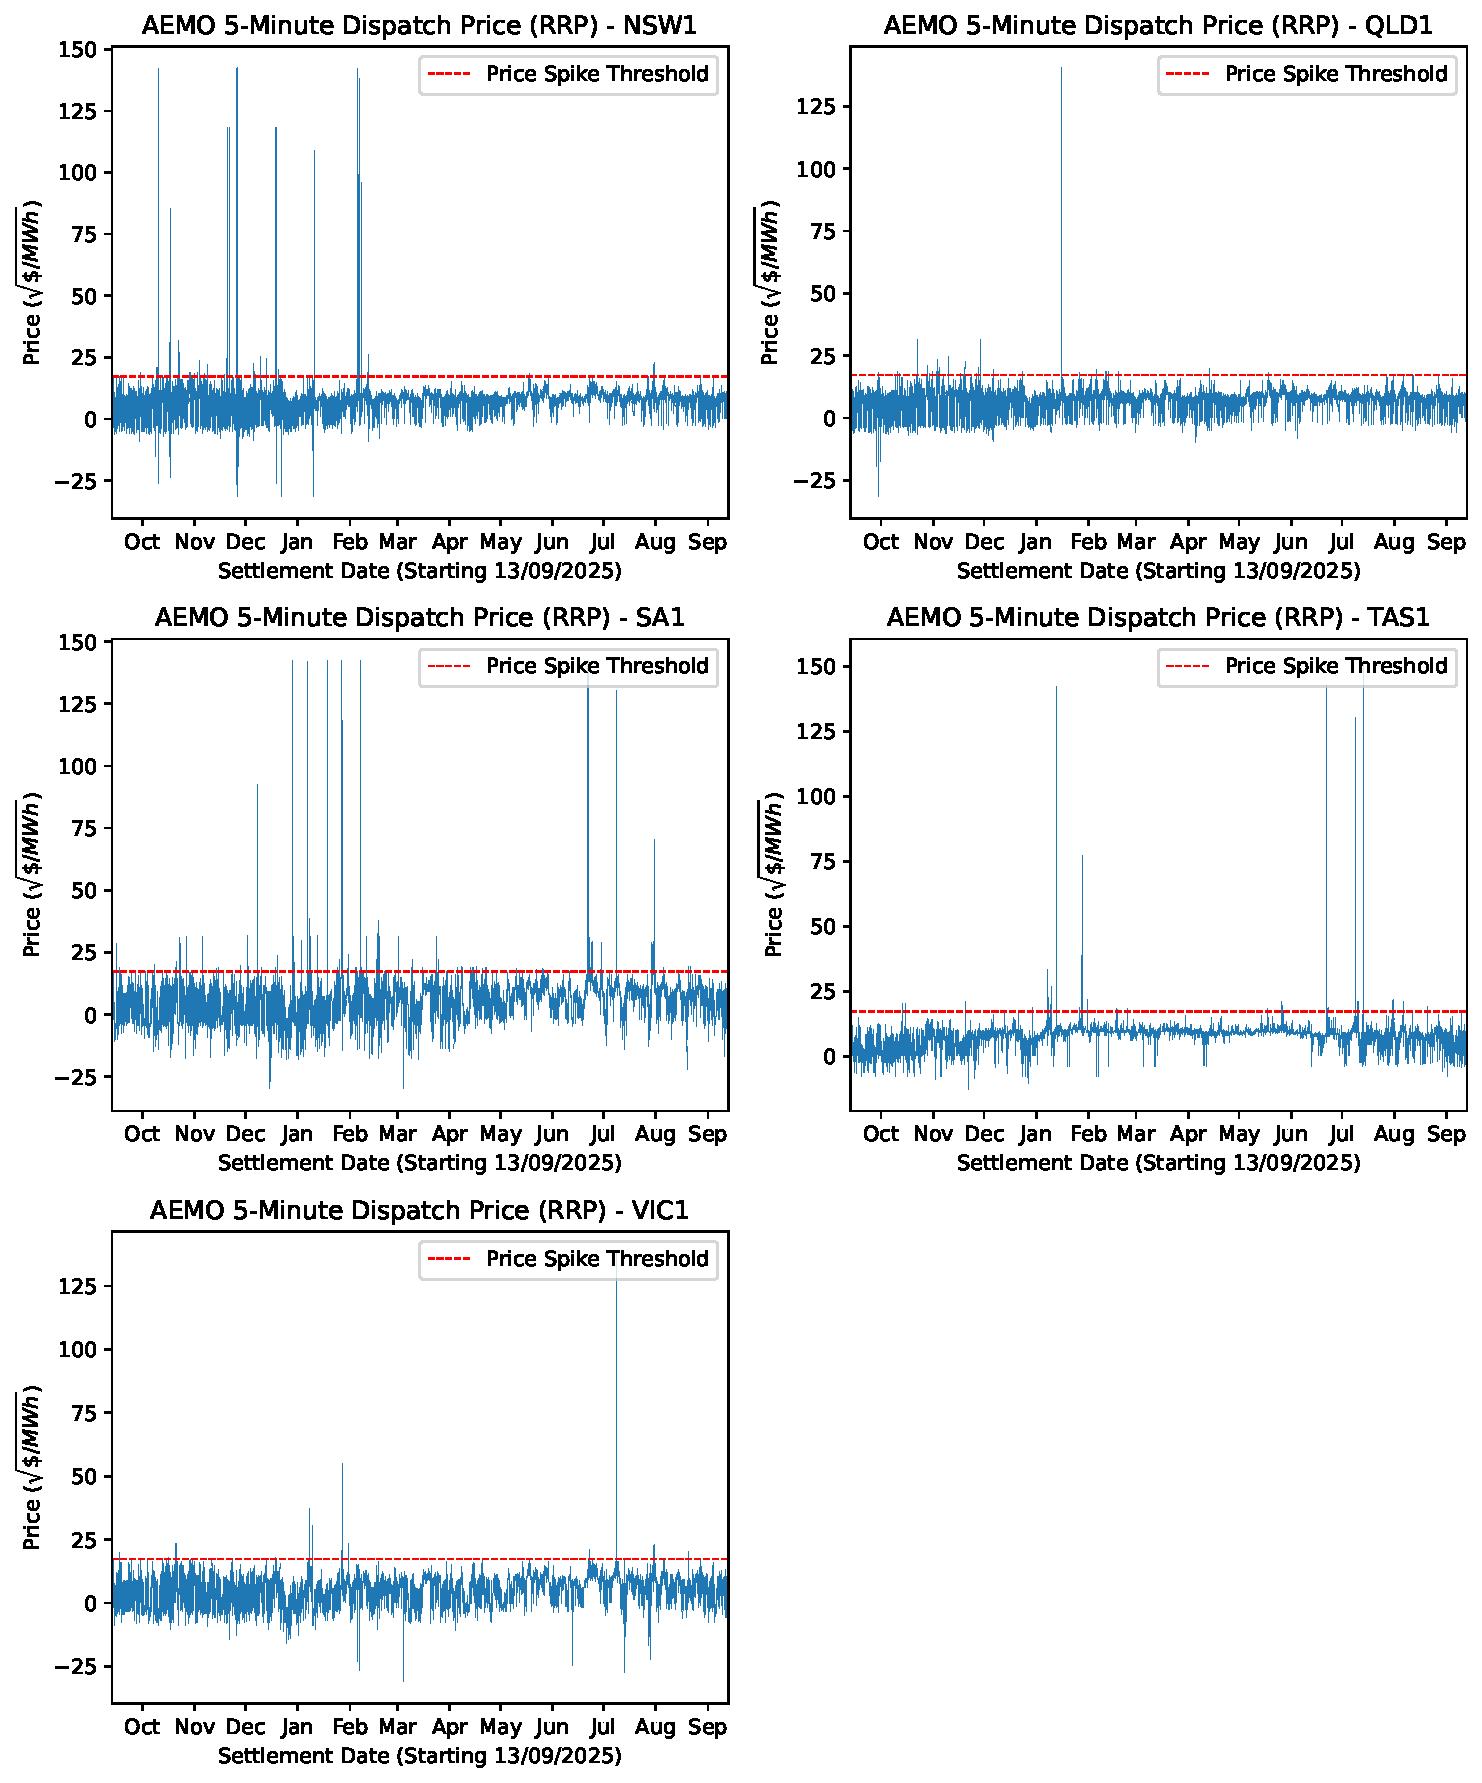
\includegraphics[width=0.85\textwidth]{price_series.pdf}
\caption{Five minute regional reference price, signed square root scale. The dashed line is the \$300/MWh threshold.}\label{fig:prices}
\end{figure}

\begin{table}[!htbp]\centering\small
\caption{Price summary by region (\$/MWh). Spike share is the fraction of intervals above \$300/MWh, and price share is the
fraction of the year's summed price earned in those intervals.}\label{tab:prices}
\resizebox{\textwidth}{!}{\begin{tabular}{lrrrrrrrr}
\toprule
 & mean & median & std & excess\_kurtosis & max & spike\_count & spike\_frac & spike\_price\_share \\
REGIONID &  &  &  &  &  &  &  &  \\
\midrule
NSW1 & 73.8 & 70.5 & 263 & 3.66e+03 & 2.03e+04 & 282 & 0.00268 & 0.0781 \\
QLD1 & 62 & 65.8 & 88.1 & 2.64e+04 & 1.97e+04 & 65 & 0.000618 & 0.00971 \\
SA1 & 70 & 50.7 & 474 & 1.55e+03 & 2.03e+04 & 1492 & 0.0142 & 0.264 \\
TAS1 & 68.1 & 78.1 & 151 & 1.61e+04 & 2.32e+04 & 152 & 0.00145 & 0.0276 \\
VIC1 & 48 & 36.8 & 93.2 & 1.81e+04 & 1.91e+04 & 220 & 0.00209 & 0.0296 \\
\bottomrule
\end{tabular}
}
\end{table}

\section{Distribution of Spikes}
Spikes are mostly an evening event, from 4pm to 9pm, when solar generation has dropped off but demand has not (Figure \ref{fig:when}).
SA1 also spikes right through the night. By month, SA1, TAS1 and VIC1 are worst in June and July (and January), while NSW1 and
QLD1 spike mostly in spring and summer. This matters for forecasting: for SA1, TAS1 and VIC1, the months the models are trained
on before the test period contain few extreme prices, and the winter test months contain many.

\begin{figure}[!htbp]\centering
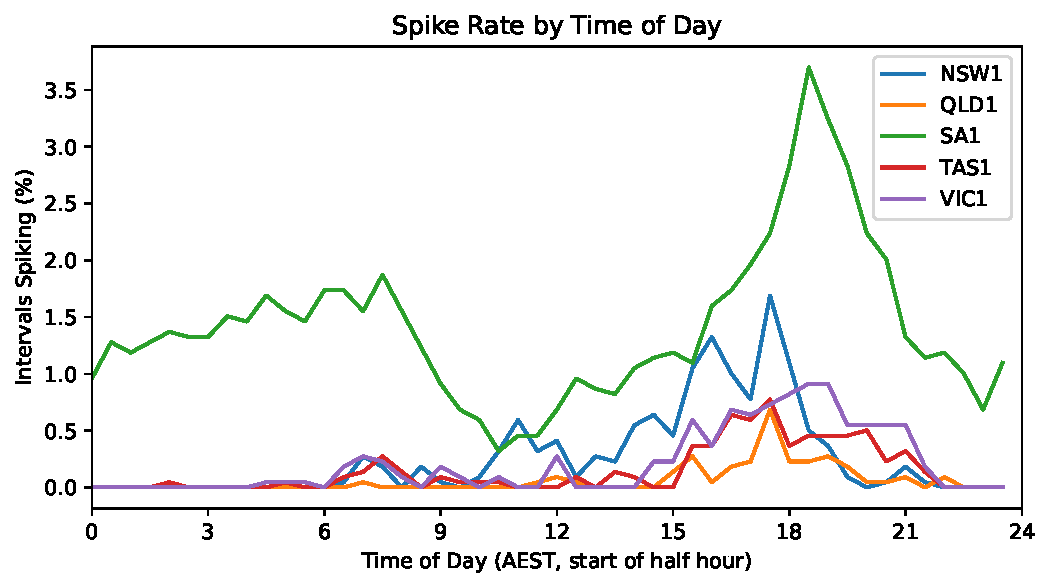
\includegraphics[width=0.62\textwidth]{diurnal_rate.pdf}\\[4pt]
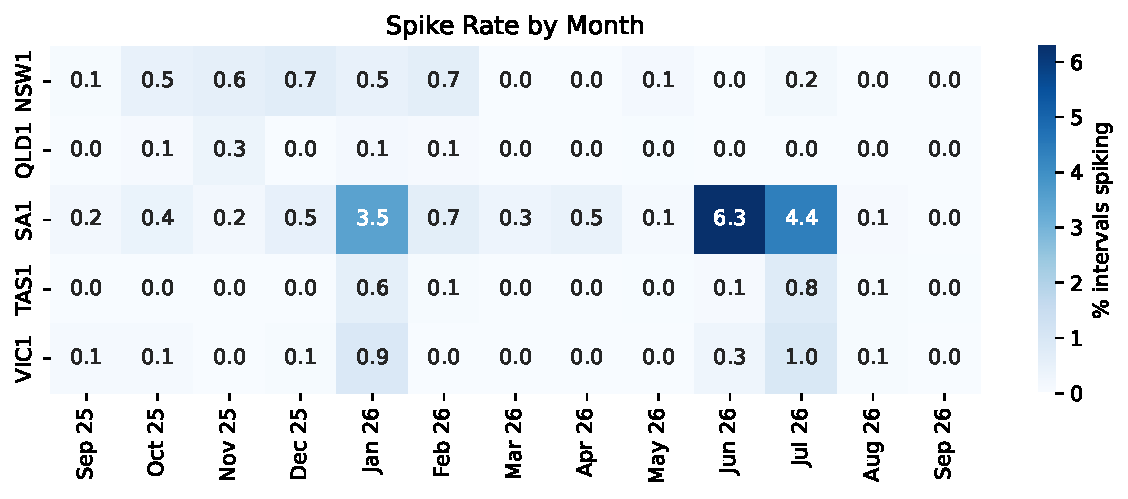
\includegraphics[width=0.95\textwidth]{monthly_rate.pdf}
\caption{Share of intervals spiking by time of day (top) and by month (bottom, \%).}\label{fig:when}
\end{figure}

\section{Episodes: how long spikes last, and how they cluster}
An \emph{episode} is a run of consecutive spike intervals, and its \emph{onset} is the first interval of the run. If spiking
were a two state Markov chain, episode lengths would be geometric, $P(L = k) = (1-q)q^{k-1}$ with $q = P_{11} = P(S_{t+1}=1 \mid S_t = 1)$,
which we test with a $\chi^2$ goodness of fit test (pooling the tail so every expected count is at least 5). If onsets were a
Poisson process, onsets per day would have variance equal to the mean, a dispersion index of 1.

Apart from QLD1, where episodes are short, the geometric law is rejected (Table \ref{tab:episodes}): long episodes are much more
common than a Markov chain allows, so once a spike has gone on for a while it is more likely to keep going. The dispersion
index is 2--8 everywhere, so onsets also cluster across days. The waiting times between onsets tell the same story
(Figure \ref{fig:waits}): compared with an exponential distribution of the same mean there are far more short waits, fewer medium
ones, and more very long ones (the quiet months). Both point to self-excitation, although part of it could also be the time of
day and season alone, which is what the Hawkes model in chapter \ref{ch:hawkes} separates.

\begin{table}[!htbp]\centering\small
\caption{Spike episodes by region. $P_{01}$ and $P_{11}$ are the Markov transition probabilities into a spike, the $\chi^2$
test is against a geometric episode length, and the dispersion is the variance to mean ratio of onsets per day.}\label{tab:episodes}
\resizebox{\textwidth}{!}{\begin{tabular}{lrrrrrrr}
\toprule
 & episodes & mean\_len\_min & max\_len\_min & P01 & P11 & chi2\_p & dispersion\_daily \\
\midrule
NSW1 & 116 & 12.2 & 165 & 0.00111 & 0.589 & 2.28e-07 & 4.54 \\
QLD1 & 53 & 6.13 & 15 & 0.000505 & 0.185 & 0.939 & 2.93 \\
SA1 & 309 & 24.1 & 1.25e+03 & 0.00298 & 0.793 & 1.01e-63 & 7.6 \\
TAS1 & 49 & 15.5 & 255 & 0.000467 & 0.678 & 6.2e-07 & 2.34 \\
VIC1 & 49 & 22.4 & 270 & 0.000467 & 0.777 & 0.000157 & 3.64 \\
\bottomrule
\end{tabular}
}
\end{table}

\begin{figure}[!htbp]\centering
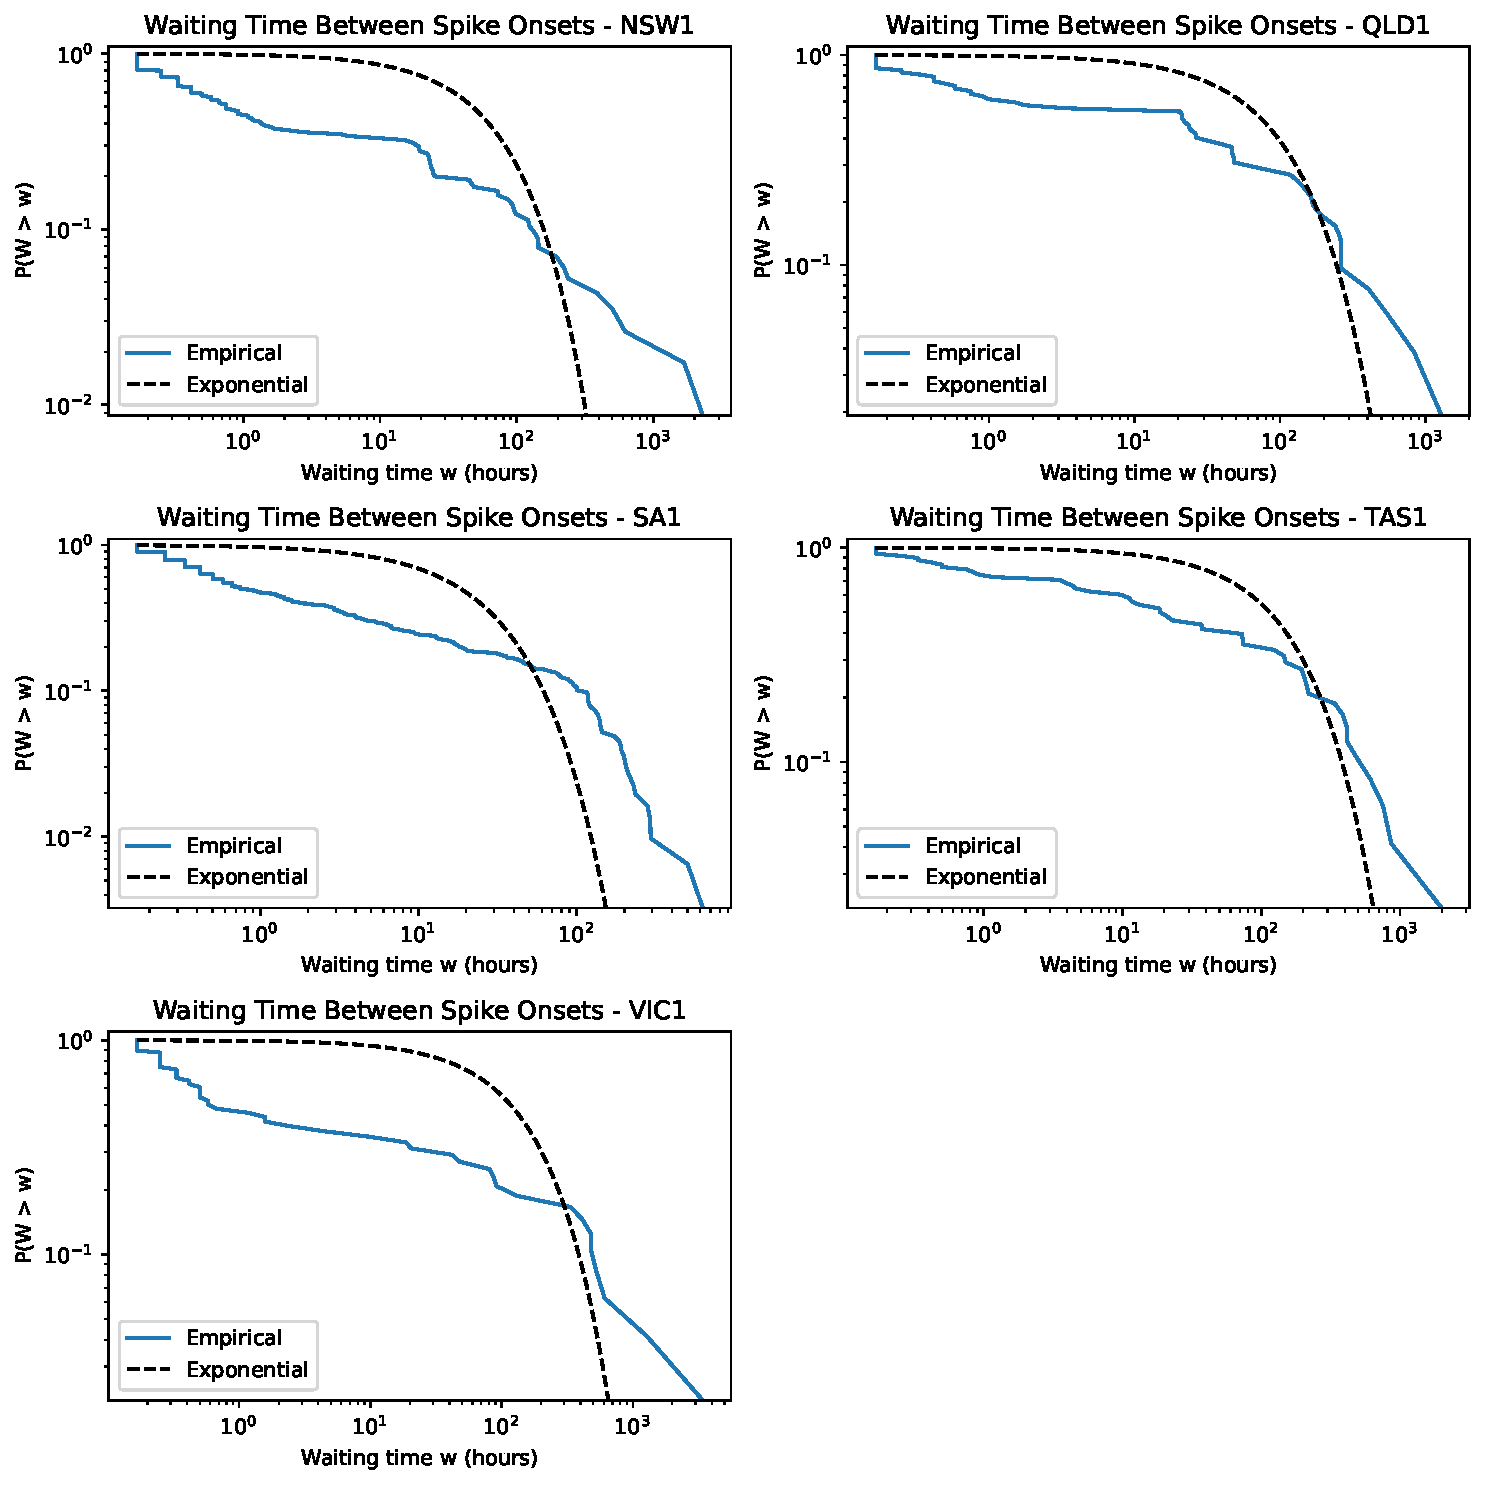
\includegraphics[width=0.8\textwidth]{interarrival.pdf}
\caption{Survival function of waiting times between spike onsets, against an exponential with the same mean.}\label{fig:waits}
\end{figure}

\section{Do regions spike together?}
We could model all spikes across the five regions as one process, but that confounds too much at once, so we model each
region separately. Figure \ref{fig:cospike} shows $P(S^j_t = 1 \mid S^i_t = 1)$. The regions split in two along the interconnectors:
NSW1--QLD1, and VIC1--TAS1--SA1. When TAS1 spikes, VIC1 is spiking too 77\% of the time, and when VIC1 or TAS1 spike, SA1 is
60--70\% of the time. QLD1 never spikes at the same time as VIC1 or TAS1. The neighbouring prices therefore go into the
forecasting models as features.

\begin{figure}[!htbp]\centering
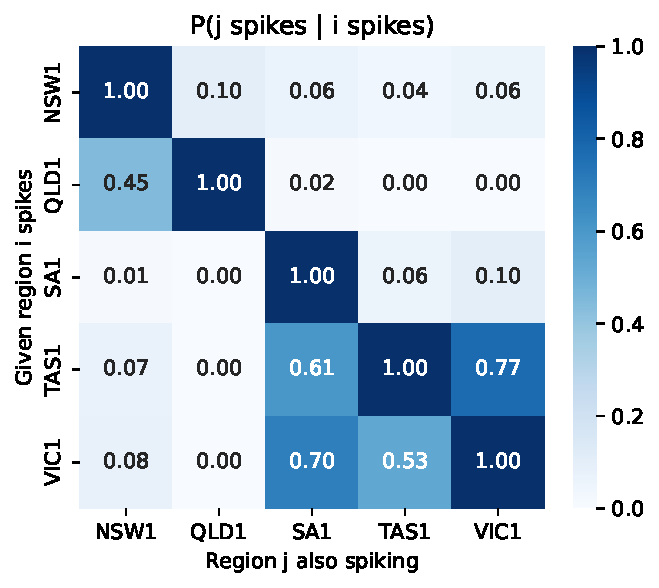
\includegraphics[width=0.5\textwidth]{cospike_matrix.pdf}
\caption{Probability that region $j$ spikes given region $i$ spikes, in the same interval.}\label{fig:cospike}
\end{figure}